\scanpage{83}
% archive foliation: 82
Les $\alpha_{p,q}$ permettent de définir des \deleted{\unsure{lois}}
\margin{\unsure{9}}
\[\unsure{\mathcal P|P}_n(X,Y)=\operatorname{Hom}_{\unsure{\mathcal P|P}_1}(\Gamma^nX,Y)\]
\inserted{donc $\left\{\begin{array}{l}\unsure{\mathcal P|P}_1(X,Y)=\operatorname{Hom}_{\unsure{\mathcal P|P}_1}(X,Y)\\P_0(X,Y)=\operatorname{Hom}_{\unsure{\mathcal P|P}_1}(1,Y)\end{array}\right.$}
et des applications
\[\begin{aligned}\unsure{\mathcal P|P}_p(X,Y)\times \unsure{\mathcal P|P}_q(Y,Z)&\longrightarrow \unsure{\mathcal P|P}_{pq}(X,Z)\\f\quad,\quad g&\longmapsto g\circ f\end{aligned}\]
par
\diagram{\begin{tikzcd}[column sep=large,row sep=large]
\Gamma^pX\arrow[r,"f"]&Y&\Gamma^qY\arrow[r,"g"]&Z\\
\Gamma^q(\Gamma^pX)\arrow[urr,"\Gamma^q(f)"]&\deleted{\unsure{\alpha}\longleftarrow\unsure{\Gamma^p(\Gamma^q(X))}\longleftarrow\Gamma}&&\\
\Gamma^{pq}(X)\arrow[u,"\alpha^X_{q,p}"]&&g\circ f=g\Gamma^q(f)\alpha^X_{q,p}&
\end{tikzcd}}
Le diagramme comm. (A) assure l'associativité de la composition, $(\unsure{u_1})$ \unsure{nous exprime|est une exigence} que si \inserted{$p=1$ ou $q=1$} \deleted{\unsure{$g$ ou $f$ est}} \deleted{de degré $1$}, alors le composé est celui provenant de la bifonctorialité des $\unsure{\mathcal P|P}_p(X,Y)$ sur $\unsure{\mathcal P|P}_1^\circ\times \unsure{\mathcal P|P}_1$, enfin la compatibilité $(\unsure{u_0})$ signifie, pour le \unsure{premier}, que
\[g\circ f=g\qquad\text{si }g\text{ de degré }0\]
le deuxième signifie
\diagram{\begin{tikzcd}[column sep=large,execute at end picture={\draw[rotate=7] (current bounding box.center) ellipse (2.5cm and .9cm);}]
\deleted{\unsure{\Gamma^0}}&\\[-1.5ex]
1\arrow[r,"\alpha_{q,0}"]&\Gamma^q(1)
\end{tikzcd}}
\margin{\unsure{pourtant}}
\figure{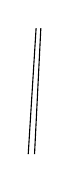
\begin{tikzpicture}\draw (0,0)--(.1,1.6);\draw (.08,0)--(.16,1.6);\end{tikzpicture}}
Je l'avais oublié dans les axiomes préliminaires il me semble, \unsure{que}\newline
\unsure{je n'} \unsure{d'avais des} \unsure{vrais} \illegible{1}

